\chapter{Forschungsstand}
\label{ch3:Forschungsstand}

\section{Gamification}
\label{ch3:s:Gamification}

Der Begriff Gamification geht auf Nick Pelling 2002 zurück.
Er beschreibt den Prozess bei dem Spielmechaniken auf bestehende Aspekte angewendet werden um eine extrinsische Motivation zu erzeugen.\citep{Marczewski.2013}
Erste Gamification Ansätze gab es zu Beginn des 20. Jahrhunderts z.\,B. durch Stempelkarten an der Eisdiele. Später wurden ähnliche Konzepte in Vielfliegerprogrammen aufgegriffen.

In der Literatur gibt es unterschiedliche Definitionen der Gamification.
In der nachfolgenden Tabelle \ref{table:ch3:lit_overview} sind verschiedene Autoren wie deren Einordnung des Gamification Begriffs zu sehen.
Es lässt sich zunächst feststellen, dass ein gemeinsamer Konsens in der Literatur darüber herrscht, dass Gamification eine Nutzung von Spielmechaniken darstellt.
Vergleicht man die einzelnen, lässt sich feststellen, dass \cite{Zichermann.2011} und \cite{Kapp.2012} eine Übereinstimmung bezüglich der Nutzung von Gamification als Motivation finden, sowie als Mittel zur Lösung von Problemen. \cite{Zichermann.2011} definiert hier die Gamification als Mittel um extrinische Motivation zu erzeugen, welche entsprechend Einfluss auf die Handlungen des Einzelnen hat.
\cite{Deterding.2011}, \cite{Breuer.2011} und \cite{Oxford.2013} grenzen dazu im Vergleich die Gamification von normalen Spielen explizit ab. Diese legen Wert darauf, dass explizit keine Spiele als Gamification verstanden werden, sondern als Basis des Gamification eine normale Tätigkeit steht.
\cite{Kapp.2012} geht im Vergleich zu den restlichen Autoren hier weiter und ergänzt die Nutzung von Gamification als Lehrmittel, stellt diese als Motivator für Personen dar. Speziell die Nutzung von Gamification im Zusammenhang der Lehre lässt sich in der aktuellen Literatur ebenfalls verflogen (Quelle!).
Gamification kann genutzt werden um ein Empowerement bei den partizipierenden Spieler zu erzeugen \cite{Jeannerod.2003}. 
Ein Beispiel für die Nutzung von Gamification stellt das Sammeln von Geinformationen mithilfe einer App dar. \citep{Odobasic.2013}

%%\begin{table}
\begin{sidewaystable}
\footnotesize
\begin{tabular}{llllll}
~ & \textcite{Zichermann.2011} & \textcite{Deterding.2011} & \textcite{Breuer.2011} & \textcite{Oxford.2013} & \textcite{Kapp.2012} \\
Nutzung von Spielmechanik & X & X & X & X & X \\
Motivation & X & ~ & ~ & ~ & X \\
Problemlösung & X & ~ & ~ & ~ & X \\
Spielferner Kontext & ~ & X & X & X & ~ \\
Verhaltensbeinflussung & ~ & ~ & X & ~ & ~ \\
Lernförderung & ~ & ~ & ~ & ~ & X \\
Anregung zum Handeln & ~ & ~ & ~ & ~ & X \\
\end{tabular}
\label{table:ch3:lit_overview}
\caption{Literaturübersicht zur Definition von Gamification}
%%\end{table}
\end{sidewaystable}

Eine Einordnung und Abgrenzung der Terminologie ist in \ref{img:ch3_img02_gamification} zu sehen.

\begin{figure}[H]
\begin{center}
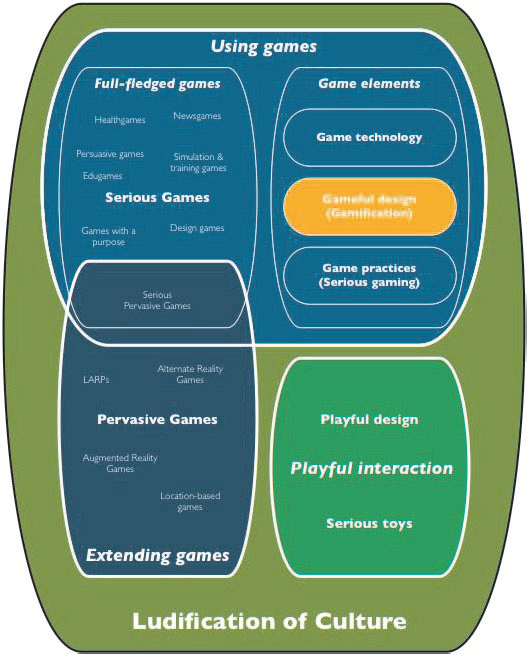
\includegraphics[width=100mm]{images/ch3_img02_gamification.png}
\caption{Gamification nach \textcite{Deterding.2011}}
\label{img:ch3_img02_gamification}
\end{center}
\end{figure}

In der Literatur werden die Elemente Points, Badges und Leaderboards (PBL) angesprochen. Diese dienen als Mittel um eine Gamification durchführen zu können. 
Points stellen Punkte dar, die verwendet werden um einen Fortschritt des einzelnen Spielers darzustellen. Dies sind zum Beispiel Meilen in Vielfliegerprogrammen oder Statuspunkte bei Bahn Bonus.
Bei Badges handelt es sich um Abzeichen, welche für bestimmte Erungenschaften an den Spieler vergeben werden. Ein Beispiel hierfür ist das Trainspotter Badget bei Foursquare, welches ausgestellt wird, wenn der Spieler in eine gewisse Anzahl von Bahnhöfen eingecheckt hat. Die Badges sollen einen gewissen Status gegenüber den restlichen Spielern suggestieren.
Leaderboards sind klassische Ranglisten. Diese dienen dazu einen Wettbwerb unter den Spielern zu erzeugen. Hierbei wird empfohlen nicht auf die klassische Top10 Liste, wie bei vielen Spielhallen Automaten zurückzugreifen. Stattdessen soll der Spieler zwischen anderen platziert werden, vorzugsweise sind die Spieler über und unter dem aktueller Spieler dessen Freunde (vgl. Foursquare). Dies verhindert, dass der Spieler von überhöhten Punktzahlen abgeschreckt wird.

\cite{Zichermann.2011} erweitern das Modell in dem es um weitere Aspekte ergänzen und mehr Struktur geben.
Sie pflegen den Begriff SAPS. Dieser unterteilt sich in Status, Access, Power und Stuff (SAPS).
Das bekannte PBL der Literatur wird unter Status zusammengefasst wie in nachfolgender Aufzählung zu sehen.

\begin{itemize}
\item Status (Badges, Levels, Leaderboards)
\item Access (early Access)
\item Power (give power, e.g. modicum control over other players)
\item Stuff (give a reward, try to prevent that the price gets known)
\end{itemize}

Bei Access handelt es sich um \glqq Zugriff \grqq zu exklusiven Dingen, welche man dem Spieler gewährt. Ein Beispiel hier für ist die Lufthansa Senator Lounge oder die DB Lounge.
Es kann sich um einen zeitlich verfrühten Zugriff auf ein Produkt oder Funktionen handeln.

Unter Power sind Mechaniken zu verstehen, welche es dem Spieler erlauben Einfluss -- Macht -- auf andere Spieler aus zu üben. Dies kann z.\,B. durch Moderationsrechte ab einem bestimmten Level realisiert werden. Foursquare realisiert dies durch Superuser.

Der letzte Punkt ist Stuff. Hierbei handelt es sich um Belohnungen die dem Spieler zuteilwerden. Klassischerweise handelte es sich hierbei z.\,B. um ein zusätzlich kostenloses Eis. Ziel ist es dem Spieler nicht einen konkreten monitären Gegenwert sehen zu lassen. D.h. dem Spieler soll es nicht ersichtlich sein wie viel der Reward wert ist. Ziel sollte es nicht sein kostenlos dem Spieler zu geben, sondern viel mehr , was seinen Status unterstreicht.\\

Im Zuge der Gamification wird gerne der Begriff des \textit{Flow}-Zustandes aufgegriffen.
Hierbei handelt es sich um einen von \cite{Csikszentmihalyi.1991} eingeführten Begriff, bei dem es darum geht den Spieler zwischen einem optimalen Zustand zwischen Anspannung und Langeweile zu halten. In dem Flow Modell wird angenommen, dass der Mensch sich in einer Situation jeweils seiner Handlungsmöglichkeiten als seiner Fähigkeiten bewusst ist.
Übersteigt der Umfang der Aufgaben die Fähigkeiten, stellt sich der Zustand oberhalb des flow Zustande ein, wie in Abbildung \ref{img:ch03_img02_flow} zu sehen. D.h. Sorge bzw. Sorge. Bei einer Unterforderung oder Einschränkung der Handlungsmöglichkeiten stellt sich schnell Langeweile ein. Das Ziel ist es den optimalen Zustand für den Spieler zu finden. Viele Spiele arbeiten unter anderem mit dynamischen Schwierigkeitsstufen (vgl. Gummi Band KI/Mario Kart).

\begin{figure}[H]
\begin{center}
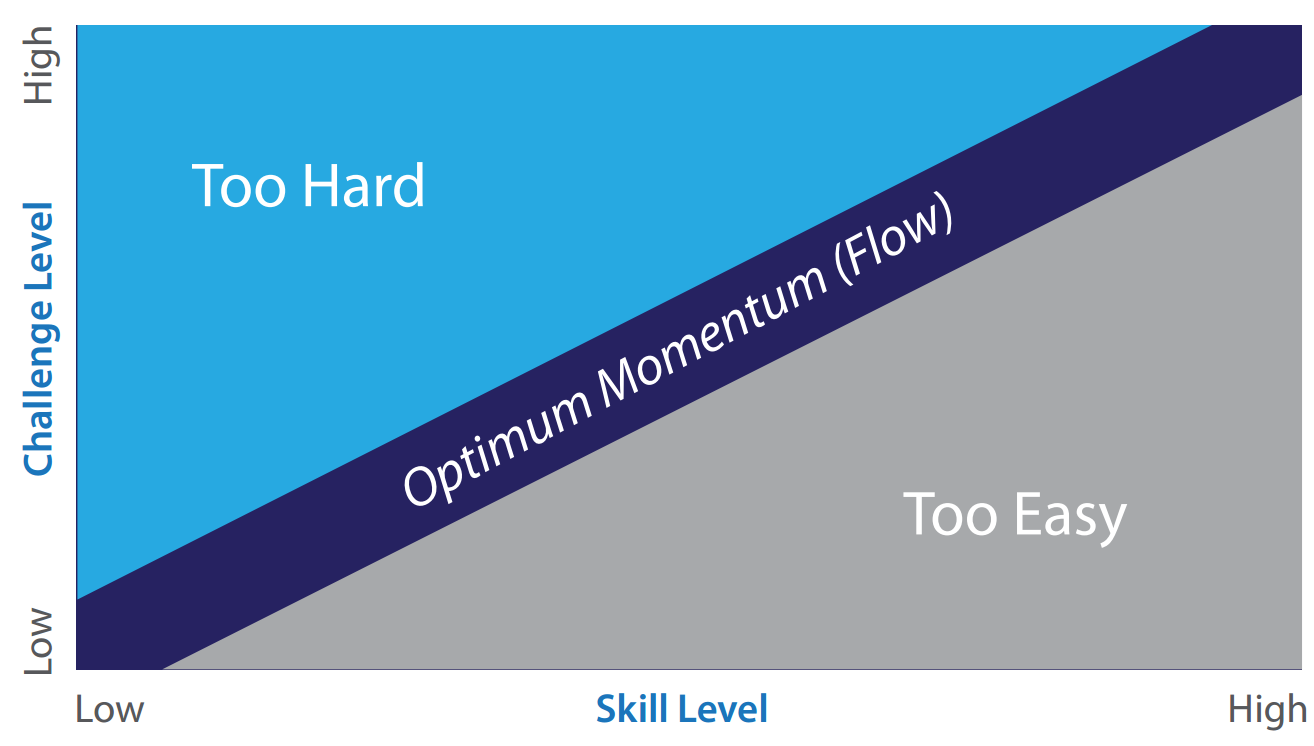
\includegraphics[width=120mm]{images/ch03_img02_flow.png}
\caption{Flow Zustand nach nach \textcite{Csikszentmihalyi.1991}}
\label{img:ch03_img02_flow}
\end{center}
\end{figure}

\section{Geogames}
\label{ch3:s:Geogames}

\subsection*{Spiel}

Um den Geogames Begriff zu klären muss zunächst abgegrenzt werden, was unter dem Begriff Spiele zu verstehen ist. In der Literatur gibt es hierfür viele Definitionen.
In diesem Kontext soll die Definition analog zu \cite{Salen.2010} verwendet werden, welche ein Spiel als Abgrenzung zum normalen Alltag darstellt. Hierbei wird ein Spiel innerhalb eines sogenannten Magic Circles durchgeführt.
Der magische Kreis dient als Regelraum in welchem das Spiel durchgeführt wird.

%\subsection*{Spielertypen}

\subsection*{Mobilegames}

Unter Mobilegames sind Spiele aller Art zu verstehen, die unterwegs gespielt werden. Diese werden auf mobilen Endgeräten gespielt. \cite{Bell.2006} Unter Mobile Endgeräte fallen klassische Handheld-Konsolen wie z.\,B. Nintendo Game Boy, Smartphones.

\subsection*{Location based Games}

Geogames sind Spiele welche in einem Geokontext gespielt werden. Hierbei wird die aktuelle Position des Spielers als Kontrollelement verwendet\citep{Schlieder.2006}. Durch dieses kann der Spieler mit den Spiel interagieren.
Geogames sind nicht begrenzt auf digitale Spiele, sondern haben Ihren Ursprung in Treasure-Hunt Games. Ein späterer Nachfolger stellt z.\,B. das Geocaching dar.
Ziel der Geogames ist die Interaktion des Spielers mit der Umgebung. Dies unterscheidet sich von den klassischen Konsolen Spielen, bei denen der Spieler die Steuerung über einen Controller welchen er per Hand steuert, bedient. Grenzt man diese motorische Steuerung ab, gibt es die Zwischenstufe des Vistaspaces. Im Vistaspace steuert der der Spieler das Spiel nicht mehr mit seinen Händen, sondern mit motorischen Bewegungen. Beispiele hierfür sind die Nintendo Wii und die Xbox Kinect. Bei diesen werden durch Lagesensoren und Infrarot Kameras die Bewegungen des Spielers erfasst und in entsprechende Spielsituationen eingebunden.
Verlässt der Spieler die eigenen vier Wände und hält sich im sogenannten environmental space.
Hierbei findet die Steuerung der Spiels durch Locomotion, d.h. der Fortbewegung des Spielers statt. \cite{Benford.2003,Kiefer.2007}

In Tabelle \ref{table:ch3:space_overview} ist eine Gegenüberstellung der einzelnen Bereiche zu sehen.

--Vergleich Vista Space, Environmental Space etc. Tabelle 3.2
Tabelle nach Schlieder/M...
\label{table:ch3:space_overview}

In der aktuellen Literatur werden vermehrt Spiele entwickelt und untersucht, die auf die Nutzung von Smartphones richten. \cite{Rashid.2006a}
Durch Integration von GPS-Modulen, den fallenden Preisen für die mobile Datenübertragung und der Vereinfachung der Entwicklung entsprechender Spiele stehen diesen einer wachsenden Zielgruppe gegenüber.

Eine Spezifizierung der der location based games stellen die sogenannten Geogames dar. Dieser Begriff wird vor allem von (Schlieder, Kiefer, May..) gepflegt. Hierbei handelt es sich vorzugsweise um klassische Brettspiele, deren Spielkonzept auf location based games übertragen werden. Die Grundidee ist es, die strategischen Reize der Brettspiele mit den ortsbezogenen Affordanzen der Echtzeit Situation von location based games zu verbinden. In diesem Zug werden rundenbasierte Spielmechanismen ausgetauscht gegen die Locomotion des Spielers. Die damit verbundenen Probleme und Schwierigkeiten werden in \cite{Schlieder.2006} beschrieben.

\subsection*{Pervasive Games}

Unter Pervasive Games sind Spiele zu verstehen, welche den in diesem Kapitel beschriebenen Magic Circle in seinen beschriebenen Dimensionen erweitern.
Konkret werden die definierten Grenzen typischer Spiele überschritten. \cite{Montola.2005}
Hierbei geht es um die Expandierung der ortsspezifischen, zeitlichen und sozialen Grenzen. \cite{Montola.2009}
Darüberhinaus gibt es in der Literatur bei Nieuwdorp(TODO) und Björk(TODO) eine weitere Dimension, welche als 'ambiguity 
of interaction or interface' definiert wird. Hierbei geht es um Unklarheit bzw. Eindeutigkeit der Interaktion.
Eine Vielzahl von Pervasive Games wurde in der Literatur behandelt und entsprechend untersucht.
Beispiele hierfür sind Can You See Me Now (Flintham et al., 2003a), GeoTicTacToe, CityPoker, Neocartographer von (Schlieder et al. 2005a, Schlieder 2005b), Human Pacman (Choetek et al. 2004) Feed my Yoshi.
Anhand dieser Spieler wurden Erketnisse in der Praxis gewonnen, welche sich in Teilen mit der Gamification Literatur in Kapitel \ref{sec:S3_Gamification} decken.
Eine Sammlung interssanter Spielkonzepte stellt die Sammlung von (Hinske et al., 2007) dar.

außerhalb der Literatur werden zunehmend Pervasive Games entwickelt.
Beispiele hierfür sind Parallel Kingdom oder Ingress vom Google Startup Niantic Project.

Unterscheidung zwischen LBG, AR MR etc?

\section{Relokalisierungsansätze}
\label{ch3:s:Relokalisierung}

Ein wichtiger Aspekt im Zuge von Pervasive Games ist der Gamecontent. Soll ein Spiel außerhalb eines fest definierten Geografischen Raums durchgeführt werden, ist es notwendig entsprechende fremde Umgebungen mit Inhalt zu füllen. \cite{Montola.2005} 
Bei der ortsbezogenen Relokation von Spielinhalten gibt es unterschiedliche Ansätze.
Zunächst müssen die ortsbezogenen Affordanzen beachtet werden. Hierbei handelt es sich um die lokalen Gegebenheiten, welche einen Einfluss auf das Spielgeschehen haben.

muss bei der Durchführung des GeoTicTacToe Spiels in Bamberg überlegt werden, inwiefern die Anordnung der 9 Spielpunkte einen Einfluss auf das Spielgeschehen hat. Brücken, Gebäude und Wege sind nicht strikt linear oder in Quadraten wie in vielen amerikanischen Städten oder z.\,B. in der Mannheimer Innenstadt. Da eine perfekte Ausgeglichenheit der Spielfelder dazu führen würde, dass jegliche Informationen über Entfernungen, Fußgängerampeln Steigung des Wegs, körperliche Verfassung des jeweiligen Spielers, sowie dessen spatiale Fähigkeiten vorhanden sein müssten, würde ein extrem komplexes Modell ohne Ideale Lösung entstehen. werden die ortsbezogenen Affordanzen als gegeben hingenommen bzw. in das Spiel als Herausforderung bzw. Spielelement integriert.

Generell gibt es drei Ansätze zur Relokation der Spielemente auf einer Karte.

\begin{itemize}
\item Keine Anpassung -- Spiel an einem Ort möglich
\item Komplette Anpassung -- Spiel an jedem Ort möglich
\item Hybride/teilweise Anpassung -- Spiel durch Eingriffe spielbar
\end{itemize}

In der Literatur werden die Probleme von Spielen wie dem Rexplorer\cite{Ballagas.2007} angesprochen, keine keine Lösungsansätze vorgeschlagen. Rexplorer enthält keine Anpassungen und ist in der Stadt Regensburg spielbar. Neben dem zugeschnittenen Geolocation Content ist der Controller explizit auf die Umgebung angepasst.
Hierbei handelt es sich um einen Art Zauberstab mit dem der Spieler mit den Elementen in der Umgebung interagieren kann. Dieser stellt ein Gehäuse dar, in dem ein Nokia E65 sowie in GPS Empfänger verbaut wurde.

Dazu gibt es im Gegensatz Spiele welche komplett Ortsunabhängig gespielt werden können.
Dies kann entweder durch ein Algorithmus bewerkstelligt werden oder durch die Tatsache, dass die Spielelemente keinen direkte Anpassung benötigen.
Spiele wie Feed my Yoshi, welche keine direkte Anpassung benötigen, haben deutliche Unterschiede im Hinblick ihrer Spielbarkeit abhängig von ihrer Umgebung. Die Autoren stellten fest, dass die Korrelation zwischen Bevölkerungsdichte und Anzahl der Wifis nicht den unterschiedlichen Teams unterschiedliche Vorteile verschaffte, sondern dies die Motivation der anderen Teams beinflusst, aufgrund des Vorteils der gegnerischen Teams.

Die letzte Möglichkeit stellt ein hybrider Ansatz dar. Bei diesem werden bestehende Spielfelder von einem gewissen geografischen Kontext auf eine andere Location übertragen. Hierbei wird unter optionaler Hilfenahme von Algorithmen ein Transfer der bestehenden Daten auf ein neues Spielfeld bewerkstelligt. Sofern

Konkrete Lösungsansätze sind in der Literatur mit der Ausnahme von \cite{Kiefer.2007}
nicht zu finden.
Der von \cite{Kiefer.2007} gewählte Ansatz zielt darauf ab ein Vergleich von verschiedenen Spielfeldern herzustellen um Spieler von verschiedener Herkunft gegeneinander antreten können. Ziel ist es den Aufwand und die Kosten des stagings dieser Spiele zu reduzieren. \citep{Kiefer.2007} identifiziert drei Quellen die zu einer Heterogenität der Spielfelder führen:

\begin{itemize}
\item spatial scale -- Unterschied in geografische Größe
\item static structure -- Unterschied in geografischer Struktur (Straßen, Höhe) 
\item dynamic conditions -- Verändernde Gegebenheiten (Wetter, GPS/GSM-Empfang, Verkehr)
\end{itemize}

Eine gewisse Heterogenität macht die Herausforderung für die Spieler interessanter, führen zu große Unterschiede zu einem unfairen und damit weniger gutem Spielerlebnis.
Generell gibt es zwei Arten von location-based Games. Zum einen örtlich begrenzte (spatial discrete) Spiele und zum anderen örtlich fortsetzende (spatial
continuous) Spiele.
Bei ersterem handelt es sich um Spiele die auf einem abgegrenzte Spielfeld durchgeführt werden und die Position des Geocontents fest auf der Karte definiert ist. Letztere sind Spielfelder, welche unbegrenzte Spielfelder haben und die Spielinteraktion zu jeder Position stattfinden kann.
Im Falle der spatial continuous Spiele ist ein bijectives Mapping der Ort nötig. Dies funktioniert gut bei offenen Flächen, bei der Verwendung von Straßen und innerhalb von Städten führt dies zu einer starken Verzerrung der Spielfelder und zu einem Mismatch zwischen Spielerfortbewegung und Lokomotion im Spiel .
Dies und die Tatsache, dass vorwiegend Geogames untersucht wurden führte dazu, dass spatial discrete Spiele im Detail untersucht wurden.
Konkret wurde das Spiel CityPoker\cite{Kiefer.2005b} in zwei verschiedenen Städten gleichzeitig gespielt. konnten beide Team der jeweiligen Städte über vordefinierte POIs miteinander interagieren. Untersucht wurde die optimale Gestaltung der Spielfelder, damit diese zwischen den Städten den kleinsten Unterschied zueinander darstellen. Zunächst wurden die POIs manuell gesetzt für beide Städte. Im Anschluss auf die Spielsitzung wurde untersucht, wie die unterschiedlichen Spielfelder optimal gelegt werden müssten um ein optimales Feld zu erhalten. Hierbei ist zu beachten, dass die Reihenfolge der POIs bei Citypoker eine Rolle spielt. Am Punkt 1 können Karten getauscht werden, welche beim anderen Team ebenfalls auf 1 liegen. \cite{Kiefer.2007} stellt für den Vergleich eine Entfernungsmatrix auf, welche er über ein Ähnlichkeitdmaß gegenüber gestellt werden.
Hierzu wird nachfolgendes Ähnlichkeitsmaß angewandt:

\begin{equation}
similarity = \frac{1}{n} \sum_{row=1}^{n} \sqrt{ \sum_{col=1}^{n} (c_{1,row,col} - c_{2,row,col})^2 }
\end{equation}

Hierbei stellen c1 und c2 jeweils die Entfernungsmatrizen der jeweiligen Spielfelder dar.
Zu beachten ist, dass die Entfernungen als direkte euklidische Luftlinie gemessen werden. Etwaige Höhenunterschiede, sowie örtliche Gegebenheiten werden hierbei aus gründen der Vereinfachung nicht beachtet. Anschließend wird das arithmetische Mittel der Durchschnittswerte der einzelnen Reihen gebildet.
Als Ergebnis wird angenommen, dass spatial discrete Spiele eine einfache
re Konfiguration erlauben wie unter anderem \cite{Benford.2005} angemerkt hat.

\begin{figure}[H]
\begin{center}
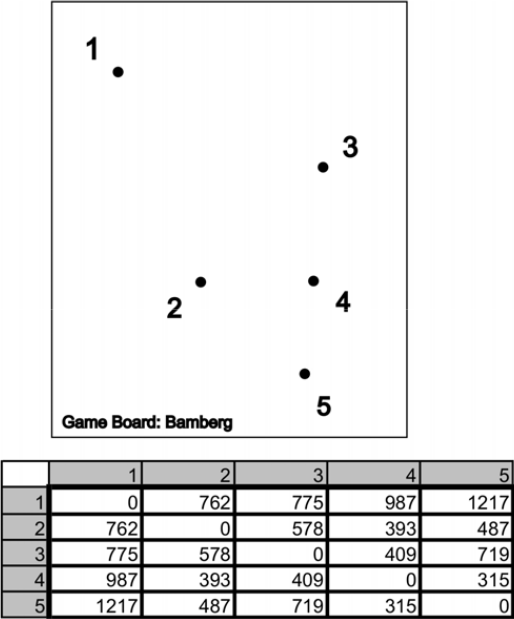
\includegraphics[width=100mm]{images/ch3_img03b_distributed.png}
\caption{Spielfeld Verteilung nach \textcite{Kiefer.2007}}
\label{img:ch03_img02_flow}
\end{center}
\end{figure}

\citep{Benford.2005} identifizieren mehrere Herausforderungen im Bezug auf spatial continous games.

\begin{itemize}
\item Hefting domains
\item Configuration
\item Orchestration
\end{itemize}

Hefting domains stellen die Problematik dar, dass Spielelemente in Computerspielen fokusiert sind auf derren virtuellen Spielwelt, müssen bei pervasive games besonderen Wert auf die Designentscheidungen bezüglich der virtuellen, reellen und hybridne Spieleelemeten gelegt werden.
Unter der Configuration ist die Adaption von pervasive games an verschiedene lokale Gegebenheiten zu sehen, d.h. die (generierte) Erstellung von Spielfeldern an anderen Orten.
Die Orchestration stellt das Management des Spiels während der Laufzeit dar. Hierbei soll sichergestellt werden, dass ein Eingriff in das Spielgeschehen zu Gunsten der Sicherheit der Spieler als des Spielerlebnisses möglich ist.

Erste Ansätze für Relokalisierung von Spielfelder lassen sich in der Literatur finden. behandeln diese erste Ansätze, wie z.\,B. \citep{Mannara.2012}, welcher eine DSL entwirft zur Nutzung von OSM Daten für das Auffinden gleicher Spielelemente (Uni Campi).

lässt sich abschließend feststellen, dass in der Literatur keine konkreten Lösungen für die (teil-)automatisierte Erstellung von Spielfeldern existiert.
An dieser Stelle soll die Arbeit des Autors ansetzten und eine Lösungsmöglichkeit präsentieren.

\section{Verwendung offener Geodaten}
\label{ch3:s:offeneGeodaten}

Zunächst ist der Begriff offene (Geo-)Daten zu definieren.
Unter offenen Daten sollen im folgenden Daten zu verstehen sein, welche unter freier Lizenz zur Verfügung stehen und somit ohne Lizenzgebühren verwendet werden können. Hierbei soll im Idealfall sowohl eine kommerzielle Nutzung als eine private Verwendung erfolgen können.
Es lassen sich generell zwei verschiedene Quellen von öffentlichen Geodaten identifizieren.
gibt es Daten von öffentlichen Behörden. Hierbei gibt es aktuell im Zuge der Open Data Bewegung \cite{Oreilly.2007} den Anspruch Daten dieser Behörden zu den Bürgern zur Verfügung zu stellen, da diese durch Steuern gesammelt erstellt wurden. Erste Ansätze lassen sich sowohl in Großstädten wie Wien \cite{Wien.2014}, Hamburg \cite{Hamburg.2014} und Berlin \cite{Berlin.2014} finden, als für ganze Länder wie Dänemark \cite{Denmark.2014}.\footnote{Eine Übersicht ist unter \url{http://www.engagedata.eu/opendatasites} (Abgerufen am 11.02.2014) zu finden. } Die Art, Qualität, sowie Umfang der Daten unterscheiden sich . 
Eine weitere Option sind offene (Geo-)Datenbanken, welche von privaten Personen durch Mapping oder externe lizenzierte Quellen zusammen getragen werden.
Beispiele entsprechender Datenbanken sind OpenStreetMap (OSM)\footnote{\url{http://OpenStreetMap.org}} und Wikimapia\footnote{\url{http://wikimapia.org}}.
Hierbei stellt sich vor allem die Frage der Qualität der Daten im Vergleich zu kommerziellen bzw. Daten von Behörden.

//TODO: Kurze generelle Info zum Aufbau von OSM -- Bild von Relations Ways und Nodes?

\begin{figure}[H]
\begin{center}
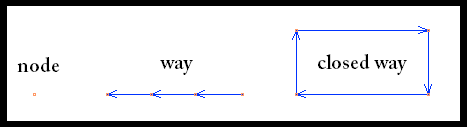
\includegraphics[width=120mm]{images/ch3_img03_OSM1.png}
\caption{OSM Elemente}
\label{img:ch03_img03_OSM1}
\end{center}
\end{figure}

In der Literatur haben sich viele Autoren mit der Qualität von OSM beschäftigt.
\cite{Haklay.2010}, \cite{Flanagin.2008} und \cite{Goodchild.2007} beschreiben, die Motivation der Personen und Problematiken, die in solchen Datenbanken entstehen. Es wird angemerkt, dass nach Ziel des Mappers eine unterschiedliche Qualitätsstufe erreicht wird.
\cite{Girres.2010} beschreibt in einem Vergleich von französischer Daten, dass die Qualität der Daten von OSM seit dem Start in 2004 enorm zugenommen hat, nach Land gibt es unterschiedliche Abdeckungssraten. haben Naturkatastrophen, einen Einfluss auf die Qualität der Daten \cite{Zook.2010}.
Zur Zeit gibt es bei OSM ca. 25.000 aktive Mapper \cite{OSM.2013}, dass Mapping in Städten ist deutlich genauer wie in den ländlichen Regionen. Generell gibt es eine Korrelation zwischen Einwohnerdichte und Datenqualität.
Die durchschnittliche Abweichung beim Vergleich von OSM zu Kartenherstellern beträgt zwischen 1 bis 30 Metern.
Darüber hinaus gibt es eine Ungenauigkeit der Namen einzelner Objekte. Diese entstehen zum einen durch die Nutzung unterschiedlicher Sprachen, durch lokale Gegebenheiten.
Die Einfachheit von OSM durch die Reduktion der Daten auf Nodes, Ways und Relations mit den dazugehörigen Tags hat den Nachteil, dass im Modell keine logische Konsistenz sichergestellt wird. Dies muss in der Verarbeitung der Daten berücksichtigt werden.
\cite{Hecht.2013} beschreibt eine geringe Covergage im Vergleich zu profesionellen Daten gibt 10\%. Dies wird von \cite{Pfoser.2013} angemerkt, wird darauf hingewiesen, dass OSM eine hohe Klassifikationsrate besitzt. Zwar stellt der Autor eine hohe Fehlerrate von 23\% fest, ist diese zu für den vernachlässigen.

Für OSM gibt es im Vergleich zu Wikmapia ausgereifte Schnittstellen. Zunächst gibt es zwei Schnittstellen direkt von OSM.
Die OSM API ermöglicht den Export der Geoinformatioenen bezogen auf eine Bounding Box. Während unter dem Namen OSM XAPI (Extended Api), es möglich ist Abfragen in Verbindung mit den zugehörigen Tags zu erstellen \cite{Meyer.2013}. Die Ergebnisse der Abfrage werden in einer XML Datei zusammengefasst.



\section{Bewertung von Spielfeldern}
\label{ch3:s:geostatistik}

Kapitel wird passend zum Evaluationskapitel gefüllt
-kNN
-cNN
